%
% LaTeX report template 
%

% This is a comment: in LaTeX everything that in a line comes
% after a "%" symbol is treated as comment

\documentclass[11pt, a4paper]{article}
\usepackage{graphicx}
\usepackage{amsmath}
\usepackage{listings}


\title{Assignment No 3} % Title

\author{Prasanna Bartakke EE19B106} % Author name

\date{\today} % Date for the report
\begin{document}		
		
\maketitle % Insert the title, author and date
\section{Data extraction and visualization}
%Create new section;it is autonumbered
The data is obtained by running the gen\_data.py script. The data contains 10 columns, the first column represents time, and the remaining 9 columns have random fluctuations with different amounts of noise where the standard deviation is uniformly sampled from a logarithmic scale. Following is the graph of all the 9 columns. 
   \begin{figure}[!tbh]
   	\centering
   	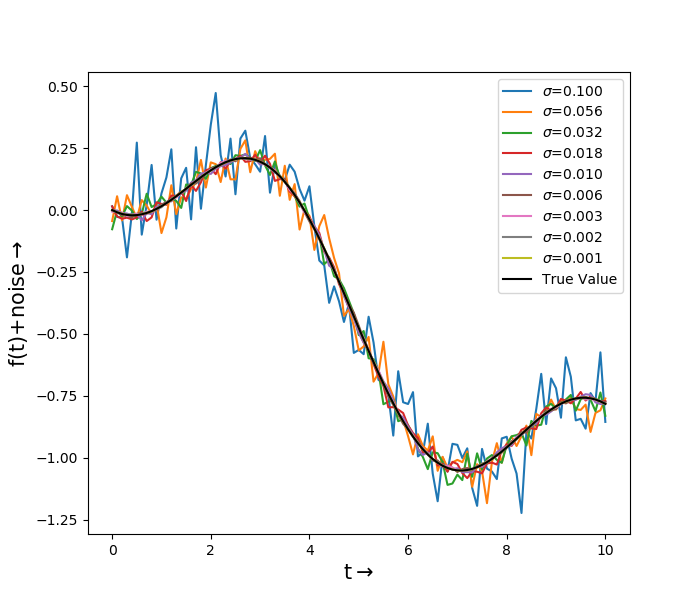
\includegraphics[scale=0.5]{data.png}  % Mention the image name within the curly braces. Image should be in the same folder as the tex file. 
   	\caption{Plot of the data}
   	\label{fig:fig1}
   \end{figure} 
\section{The Errorbar plot}
The errorbars for the first data column are plotted using the
errorbar() function. The graph is obtained by plotting every 5th data point
with errorbars and the original data. Each point in the data column is varying mostly within a $\sigma$ width of the true value.
\begin{figure}[!tbh]
   	\centering
   	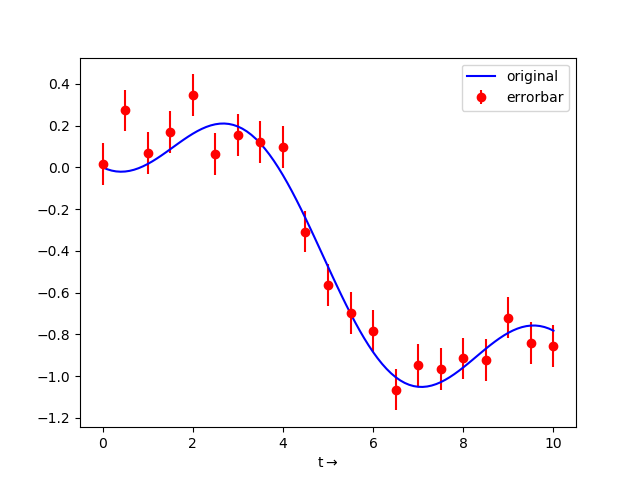
\includegraphics[scale=0.5]{errorbar_plot.png}  % Mention the image name within the curly braces. Image should be in the same folder as the tex file. 
   	\caption{The errorbar plot}
   	\label{fig:fig2}
   \end{figure} 
   
\section{Calculating the error}
The error is calculated and stored in the array e.
\begin{equation}
  \epsilon_{ij} = \frac{1}{101}\sum_{k=0}^{101}(f_k - g(t_k, A_i, B_j))^2)
\end{equation}{}
The mean squared error for the first data column can now be plotted and the minima can be found to obtain the best estimate for A and B. This is done by the following code block : 
\begin{verbatim}	
pylab.contour(A,B,e[:,:,0])
a = np.unravel_index(np.argmin(e[:,:,0]),e[:,:,0].shape)
pylab.plot(A[a[0]],B[a[1]],’o’,markersize=3)
\end{verbatim}

\begin{figure}[!ht]
   	\centering
   	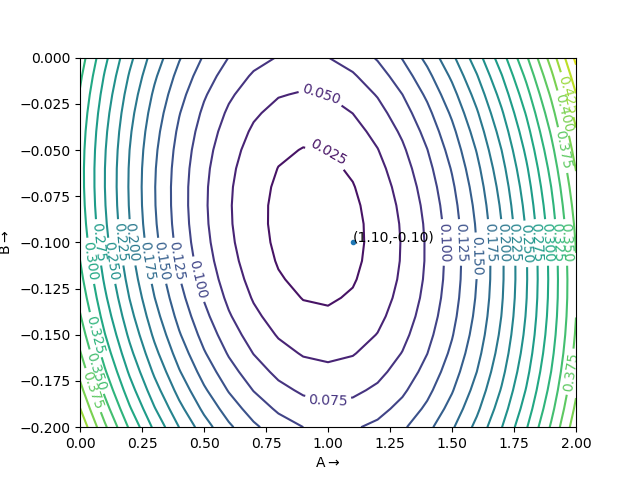
\includegraphics[scale=0.5]{contour_plot.png}  % Mention the image name within the curly braces. Image should be in the same folder as the tex file. 
   	\caption{The contour plot}
   	\label{fig:fig3}
\end{figure} 
The np.argmin() function returns the index of minima for the flattened
array, and the np.unravel index() function is used to get the location
of the minimum in the original array.


   
 As we can see in the graph, the error function has one minimum and it occurs at A = 1.10 and B = -0.10


\section{Error in estimation of the parameters}

\begin{figure}[!ht]
   	\centering
   	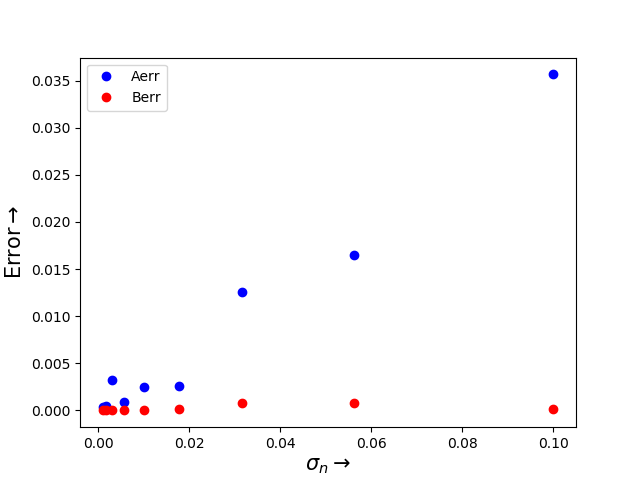
\includegraphics[scale=0.5]{error_vs_sigma_plot.png}  % Mention the image name within the curly braces. Image should be in the same folder as the tex file. 
   	\caption{Error vs $\sigma$}
   	\label{fig:fig4}
\end{figure}

\begin{figure}[!ht]
   	\centering
   	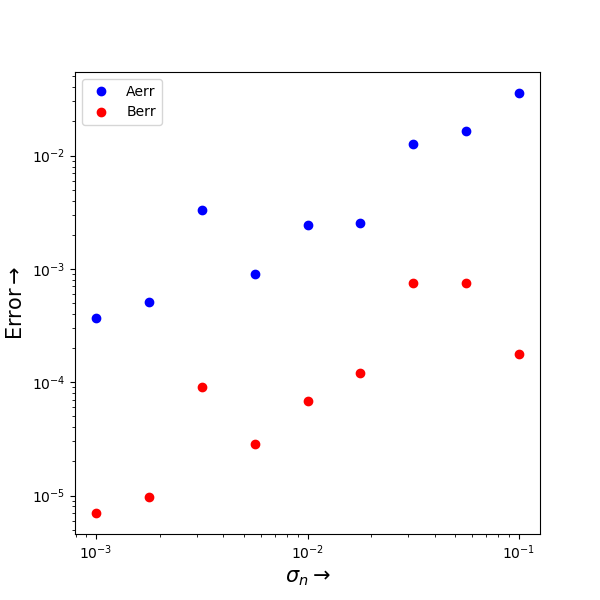
\includegraphics[scale=0.5]{error_vs_sigma_plot_log_scale.png}  % Mention the image name within the curly braces. Image should be in the same folder as the tex file. 
   	\caption{Error vs $\sigma$(log scale)}
   	\label{fig:fig5}
\end{figure}

The error estimate in the first plot is non-linear with respect to the noise.
On plotting the axes in the log scale, the graph becomes approximately linear.

\section{Conclusion}
The data with some noise is extracted and the best possible estimate for the
underlying model parameters is found by minimizing the mean squared
error.
We can see that the error is approximately linear with $\sigma$ in the
log scale.
\end{document}



 